\subsection{Static and Dynamic Kalman Filter}
First, the general static and dynamic Kalman filter will be derived. The one step prediction of the Kalman filter is given by
\begin{equation}
    \begin{gathered}
        R_{e,k}=C\,P_{k|k-1}\,C^T+R\\
        K_{fx,k}=P_{k|k-1}\,C^T\,R_{e,k}^{-1}\\
        P_{k+1|k}=A\,P_{k|k}\,A^T+G\,Q_{k|k}\,G^T-K_{fx,k}\,R_{e,k}\,K_{fx,k}^T
    \end{gathered}
\end{equation}
Where $R_e$ is the covariance of the measurement noise, $K_{fx}$ is the Kalman filter gain, $P$ is the covariance of the states and $Q_{k|k}$ can be determined by
\begin{equation}
    Q_{k|k}=Q-S\,R_{e,k}^{-1}\,R_{e,k}\,(S\,R_{e,k}^{-1})^T
\end{equation}
Q is the state noise, and is determined by \cref{eq:Q} and $S$ is the correlation between the states. In this assignment, the correlation is assumed to be 0, causing $S=0$. It is clearly then seen that $Q_{k|k}=Q$, which simplified is determined as.
\begin{equation}
    \begin{bmatrix}
        \phi_{11} & \phi_{12} \\ \phi_{21} & \phi_{22}
    \end{bmatrix}=
    \text{exp}\left(\begin{bmatrix} 
        -A_c & G_c\,G_c^T\\ 0 & A_c^T 
    \end{bmatrix}\,T_s\right)
    \qquad
    Q=\phi_{22}^T\,\phi_{12}
    \label{eq:Q}
\end{equation}
$P_{k+1|k}$ converges to the matrix $P$ (as $t\xrightarrow{}\infty$) which is the solution to the discrete algebraic Riccati equation (\textit{DARE}). The finite elements in the one step prediction can be determined as:
\begin{equation}
    \begin{gathered}
        R_{e}=C\,P\,C^T+R\\
        K_{fx}=P\,C^T\,R_{e}^{-1}\\
        P=A\,P\,A^T+G\,Q\,G^T-K_{fx}\,R_{e}\,K_{fx}^T
    \end{gathered}
\end{equation}
The general dynamic and static Kalman filter algorithm can be seen in \cref{tab:Kalman_gen}. Notice this algorithm is adjusted relating to the assumption of $S=0$, resulting in the filter gain to  become 0.\\
Since the disturbance is unknown, the system should be augmented in order to properly estimate the states. This leads the state space model of the system to take the following form. 
\begin{equation}
    \begin{gathered}
        x(k+1)=A_{aug}\,x(k)+B_{aug}\,u(k)+G_{aug}\,d(k)\\
        y(k)=C_{aug}\,x(k)+v(k)\\
    \end{gathered} 
\end{equation}
It is seen, that the unknown disturbances are stochastic variables $d(k)=N(0,\sqrt{Q})$.  The augmented matrices is determined according to \cref{eq:aug}. Notice, that also the state noise matrix $Q$ likewise is augmented.
\begin{equation}
    A_{aug}=\begin{bmatrix} A_k & E_k \\ 0 & I \end{bmatrix} \quad
    B_{aug}=\begin{bmatrix} B_k \\ 0 \end{bmatrix} \quad
    G_{aug}=\begin{bmatrix} G_k \\ 0 \end{bmatrix} \quad
    C_{aug}=\begin{bmatrix} C & 0 \end{bmatrix} \quad
    Q_{aug}=\begin{bmatrix} Q & 0 \\ 0 & I \end{bmatrix}
    \label{eq:aug}
\end{equation}
The augmented states is used in the Kalman algorithm. Notice that some of the steps in the algorithm is similar for both the static and dynamic filter. 
\begin{table}[H]
    \centering
    \begin{tabular}{c|c|c}
         & Dynamic & Static\\
        Measurement noise & $R_{e,k}=C_{aug}\,P_{k|k+1}\,C_{aug}^T+R$ & $R_{e}=C_{aug}\,P\,C_{aug}^T+R$\\
        Filter gain & $K_{fx,k}=P_{k|k+1}\,C_{aug}^T\,R_{e,k}^{-1}$ & $K_{fx}=P\,C_{aug}^T\,R_e^{-1}$\\
        Measurement update & \multicolumn{2}{c}{$y_{k|k-1}=C\,x_{k|k-1}+v_k$} \\
        Estimated measurement & \multicolumn{2}{c}{$\hat{y}_{k|k-1}=C_{aug}\,\hat{x}_{k|k-1}+v_k$}\\
        Error & \multicolumn{2}{c}{$e_k=y_k-\hat{y}_{k|k-1}$} \\
        Estimated states & $\hat{x}_{k|k}=\hat{x}_{k|k-1}+K_{fx,k}\,e_k$ & $\hat{x}_{k|k}=\hat{x}_{k|k-1}+K_{fx}\,e_k$ \\
        One step prediction & \multicolumn{2}{c}{$\hat{x}_{k+1|k}=A_{aug}\,\hat{x}_{k|k}+B_{aug}\,u_{k|k}+G_{aug}\,d_{k|k}$} \\
        Filtered state  & $P_{k|k}=P_{k|k-1}-K_{fx,k}\,R_{e,k}\,K_{fx,k}$ & $P_{\infty}=P-K_{fx}\,R_{e}\,K_{fx}$\\
        Covariance prediction step & $P_{k+1|k}=A_{aug}\,P_{k|k}\,A_{aug}^T+G_{aug}Q_{aug}G_{aug}^T$ & $P$
    \end{tabular}
    \caption{Generel Kalman filter algorithm}
    \label{tab:Kalman_gen}
\end{table}
Further more, it should be noted that the filter gain in order to minimize the noise ($K_{fw,k}$) is not shown, since it is 0, due to the fact that $S=0$ (no correlation of the state noise).
\subsubsection{Deterministic model}
For the deterministic model, the proces noise and measurement noise is 0, however the covariance of the measurement noise shall be $R>0$, in order to find a solution to the \textit{DARE}.
\begin{table}[H]
    \centering
    \begin{tabular}{c|c|cc}
         & Dynamic &\hspace{10mm} &Static\\
        Measurement noise & $R_{e,k}=C_{aug}\,P_{k|k+1}\,C_{aug}^T+R$ & & $R_{e}=R$\\
        Filter gain & $K_{fx,k}=P_{k|k+1}\,C_{aug}^T\,R_{e,k}^{-1}$ & &$K_{fx}=0$\\
        Measurement update & \multicolumn{3}{c}{$y_{k|k-1}=C\,x_{k|k-1}$} \\
        Estimated measurement & \multicolumn{3}{c}{$\hat{y}_{k|k-1}=C_{aug}\,\hat{x}_{k|k-1}$}\\
        Error & \multicolumn{3}{c}{$e_k=y_k-\hat{y}_{k|k-1}$} \\
        Estimated states & \multicolumn{3}{c}{$\hat{x}_{k|k}=\hat{x}_{k|k-1}$} \\
        One step prediction & \multicolumn{3}{c}{$\hat{x}_{k+1|k}=A_{aug}\,\hat{x}_{k|k}+B_{aug}\,u_{k|k}+G_{aug}\,d_{k|k}$} \\
        Filtered state  & $P_{k|k}=P_{k|k-1}-K_{fx,k}\,R_{e,k}\,K_{fx,k}$ & &$P_{\infty}=0$\\
        Covariance prediction step & $P_{k+1|k}=A_{aug}\,P_{k|k}\,A_{aug}$ & &$0$
    \end{tabular}
    \caption{Kalman filter algorithm deterministic system}
    \label{tab:Kalman_det}
\end{table}
\subsubsection{Stochastics model (piecewise constant)}
The algorithm for the dynamic and static Kalman filter is seen below.
\begin{table}[H]
    \centering
    \begin{tabular}{c|c|c}
         & Dynamic & Static\\
        Measurement noise & $R_{e,k}=C_{aug}\,P_{k|k+1}\,C_{aug}^T+R$ & $R_{e}=C_{aug}\,P\,C_{aug}^T+R$\\
        Filter gain & $K_{fx,k}=P_{k|k+1}\,C_{aug}^T\,R_{e,k}^{-1}$ & $K_{fx}=P\,C_{aug}^T\,R_e^{-1}$\\
        Measurement update & \multicolumn{2}{c}{$y_{k|k-1}=C\,x_{k|k-1}+v_k$} \\
        Estimated measurement & \multicolumn{2}{c}{$\hat{y}_{k|k-1}=C_{aug}\,\hat{x}_{k|k-1}+v_k$}\\
        Error & \multicolumn{2}{c}{$e_k=y_k-\hat{y}_{k|k-1}$} \\
        Estimated states & $\hat{x}_{k|k}=\hat{x}_{k|k-1}+K_{fx,k}\,e_k$ & $\hat{x}_{k|k}=\hat{x}_{k|k-1}+K_{fx}\,e_k$ \\
        One step prediction & \multicolumn{2}{c}{$\hat{x}_{k+1|k}=A_{aug}\,\hat{x}_{k|k}+B_{aug}\,u_{k|k}+G_{aug}\,d_{k|k}$} \\
        Filtered state  & $P_{k|k}=P_{k|k-1}-K_{fx,k}\,R_{e,k}\,K_{fx,k}$ & $P_{\infty}=P-K_{fx}\,R_{e}\,K_{fx}$\\
        Covariance prediction step & $P_{k+1|k}=A_{aug}\,P_{k|k}\,A_{aug}^T+G_{aug}Q_{aug}G_{aug}^T$ & $P$
    \end{tabular}
    \caption{Kalman filter algorithm stochastic system}
    \label{tab:Kalman_stoc}
\end{table}
\subsubsection{Simulation of Kalman Filter}
A simulation of the Kalman filter performance can be seen below. For the simulation, the system is initialized from the steady state where $u=\begin{bmatrix} 300 & 300 \end{bmatrix}^T$ and $d=\begin{bmatrix} 250 & 250 \end{bmatrix}^T$, with a step on the input of 10\% and the noise for the stochastic model is modelled as piecewise constant, where the covariance $Q$, the measurement noise covariance $R$ and the stochastic disturbance covariance $R_G$ has the following values (with $T_s=15[\text{sec}]$).
\begin{equation}
    Q=\begin{bmatrix}
        0.1152 & 0 & 1.0314 & 0\\
        0 & 0.0994 & 0 & 0.9653\\
        1.0314  & 0 & 12.7341 & 0\\
        0 & 0.9653 & 0 & 12.8971
    \end{bmatrix} \qquad R=0.5 \qquad R_G=5
\end{equation}
\begin{figure}[H] 
    \centering
    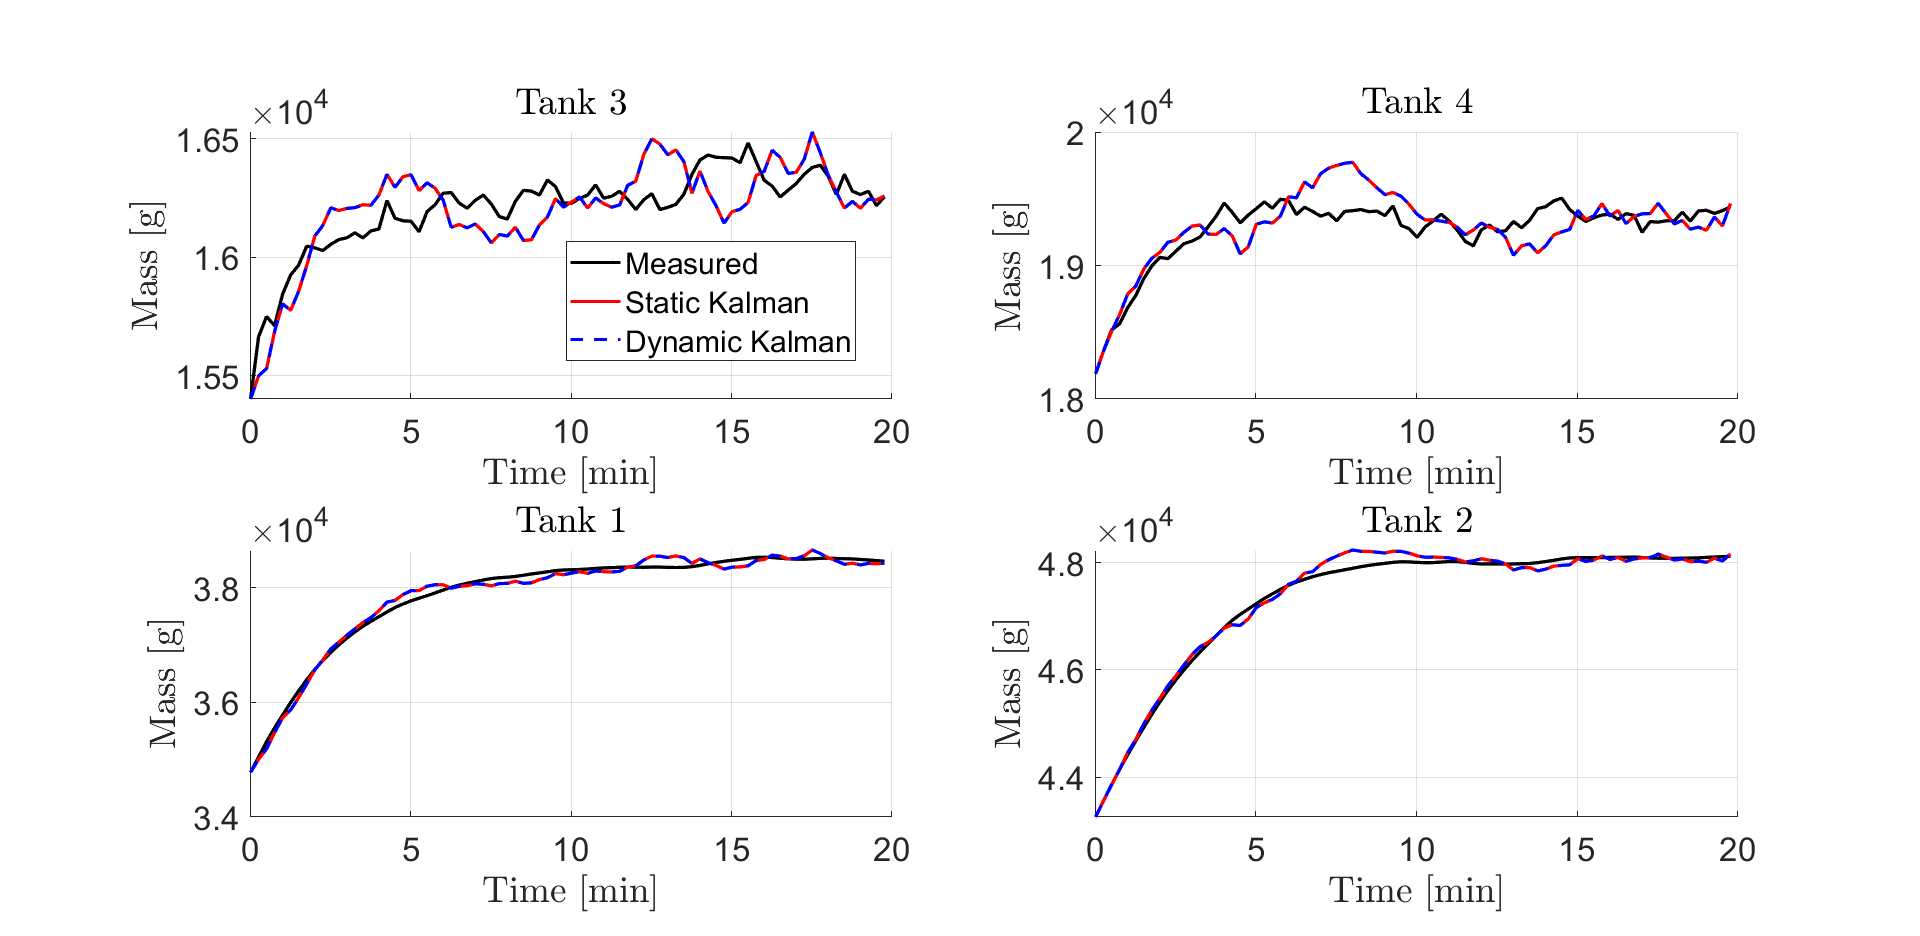
\includegraphics[width=1\textwidth]{Figures/Pr5.2_stoc_states.png}
    \caption{Kalman filter - Stochastic model states}
    \label{fig:Kalman_stoc_state}
\end{figure}
In the above figure, the states (mass in each tank) is shown. Notice, that the states is not affected directly by the measurement noise and therefore it is not shown here. It is clearly seen, that the estimate of tank 3 and 4 is poor in the beginning compared to tank 1 and 2. The reason for this, is that the system do not have a measurement of tank 3 and 4, as for tank 1 and 2 which is used to correct the estimates. The response of the dynamic and static Kalman filter is more less the same.\\
\begin{figure}[H]
    \centering
    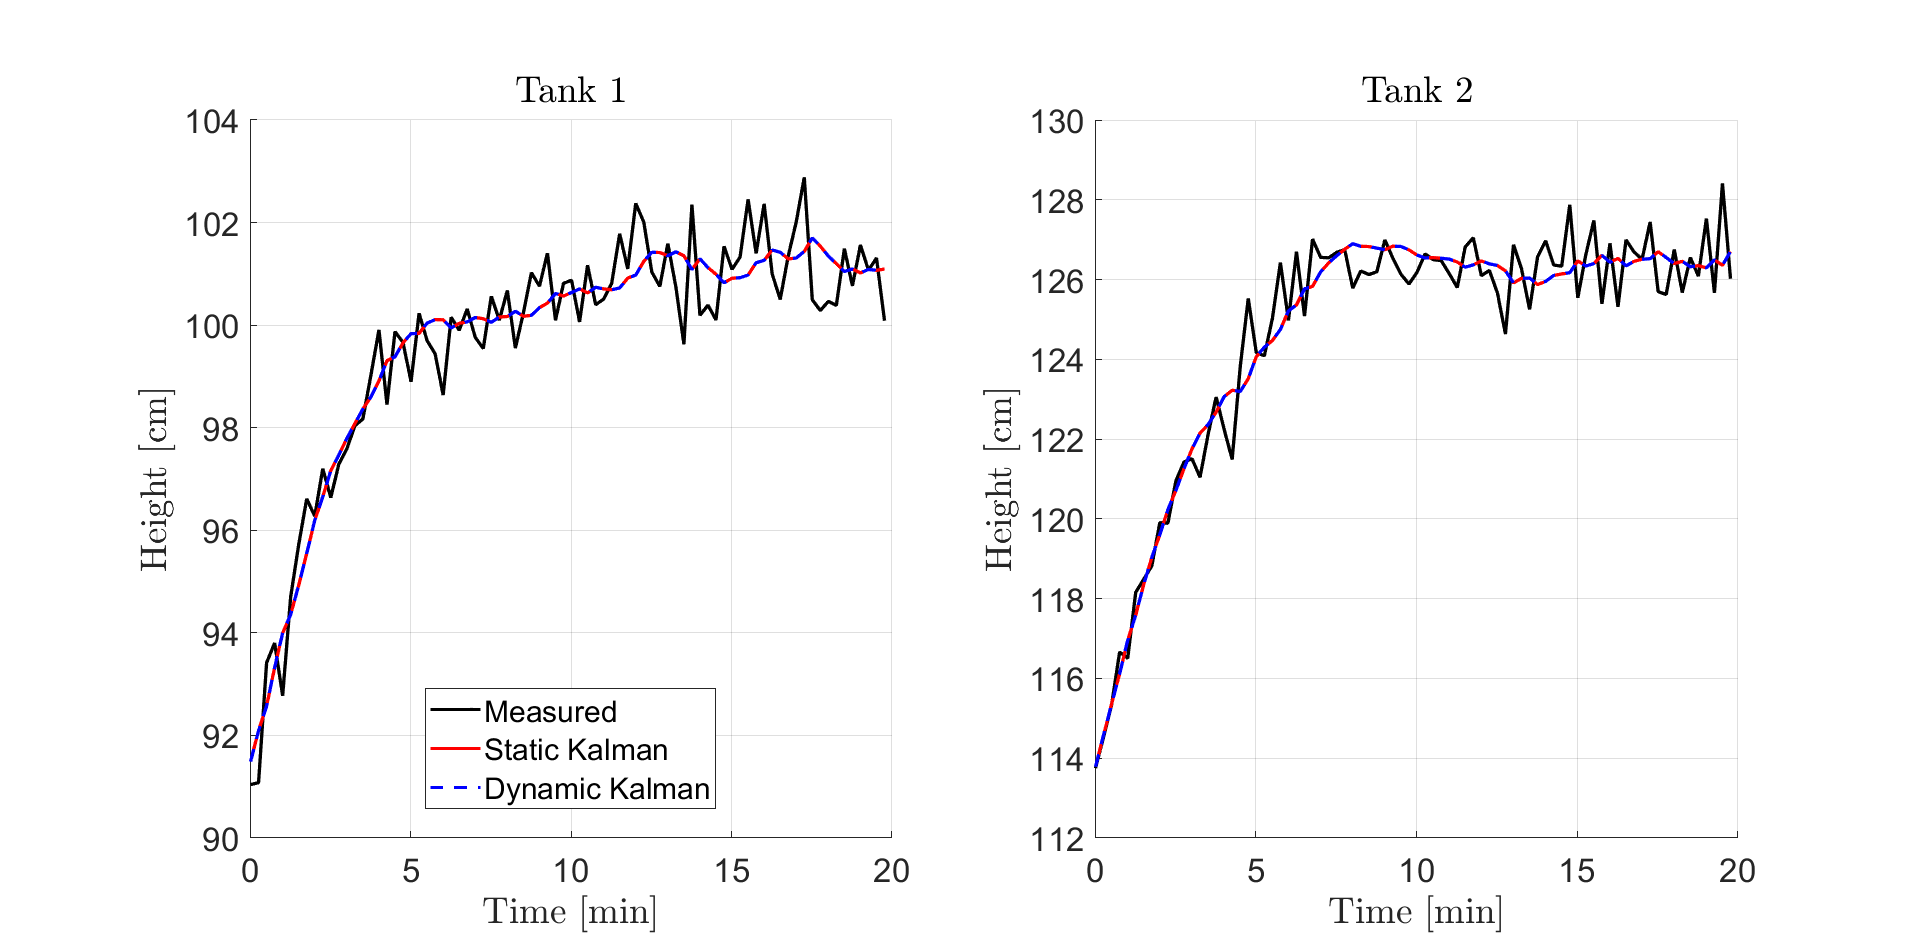
\includegraphics[width=1\textwidth]{Figures/Pr5.2_stoc_output.png}
    \caption{Kalman filter - Stochastic model outputs}
    \label{fig:Kalman_stoc_output}
\end{figure}
In the above figure, the measured output and the estimated outputs is shown. Is is clearly seen that the measured values are corrupted by the measurements noise. The Kalman filter is able to estimate the output relatively well despite the noise.